Aplikacja konsolowa do zarządzania domem służy jako aplikacja odpowiedzialna za wszystkie działania związane z Raspberry Pi oraz jego peryferiami. Na te zadania składają się 2 czynności:
\begin{itemize}
\item odczyt wartości sensorów,
\item detekcja ruchu.
\end{itemize}
Obie czynności wykonywane są niezależnie od siebie. Funkcja wykrywania ruchu działa bez przerwy, w przypadku problemu zostanie ponownie uruchomiona po około minucie za pomocą zadania wpisanego do serwisu Crontab. Odczyt parametrów wskazywanych przez czujniki odbywa się cyklicznie co 1 minutę.

\section{Odczyt wartości sensorów}
Proces zbierania danych z sensorów rozpoczyna się od pobrania odczytów z czujnika DHT11. Raspberry komunikuje się z czujnikiem za pomocą protokołu 1-wire. Do pobrania wartości wykorzystano bibliotekę dedykowaną dla tego czujnika i języka Python. Po prawidłowym odczycie, każdy z parametrów (temperatura i wilgotność) zostaje zapisany w bazie danych z odpowiednim opisem. W kolejnym kroku odczytane wartości zostają porównane z wcześniej zdefiniowanym zakresem, który jest zapisany w bazie danych. W przypadku przekroczenia lub zbyt niskiej wartości system podejmie decyzję o utworzeniu nowego powiadomienia, które będzie widoczne an stronie opisanej w rozdziale \ref{notifications}
\begin{figure}[H]
	\centering
	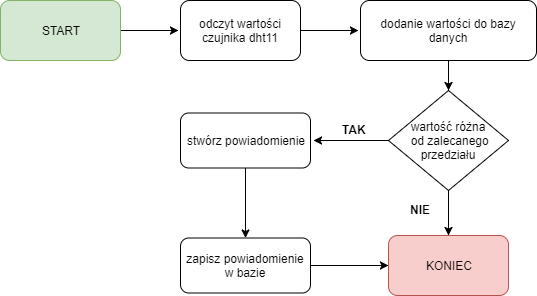
\includegraphics[scale=0.6]{odczyt_czujnikow.png}
	\caption{Proces pobierania danych z sensorów zaimplementowany w aplikacji konsolowej do zarządzania domem}
	\label{fig:odczyt_sensorow}
\end{figure}

\section{Proces detekcji ruchu}
Proces detekcji ruchu rozpoczyna się od podstawowej rzeczy, którą jest uruchomienie kamery. Jeśli kamera została uruchomiana i daje możliwość pobierania pojedynczych klatek to zostaje uruchomiona nieskończona pętla, której pierwszym krokiem jest uchwycenie najnowszej klatki obrazu. Następnie klatka zostaje przekazana specjalnej funkcji identyfikującej czy nastąpiły jakieś przemieszczenia względem poprzedniego obrazu. Proces ten został dokładnie opisany w rozdziale \ref{ss:wykrywanie}.

Jeśli moduł wykrył ruch to licznik detekcji zostaje zwiększony o 1, a w przeciwnym wypadku licznik zostaje wyzerowany. Żadne dodatkowe funkcje nie są wykonywane, aż do czasu osiągnięcia wartości równej 8 przez licznik. Liczba 8 została wyznaczona w celu ograniczenia ilości przechwytywanych ruchów do tych kilkukrotnie potwierdzonych.

Po osiągnięciu tej wartości program ostatecznie stwierdza, że nastąpił ruch i przekazuje uchwycony moment do funkcji zapisującej, której działanie opisano w kolejnej części tego rozdziału. Po udanym wykryciu licznik zostaje wyzerowany. Proces ten powtarza się tak długo, aż nie zostanie ręcznie zatrzymany poprzez wciśnięcie klawisza 'q'.
\begin{figure}[H]
	\centering
	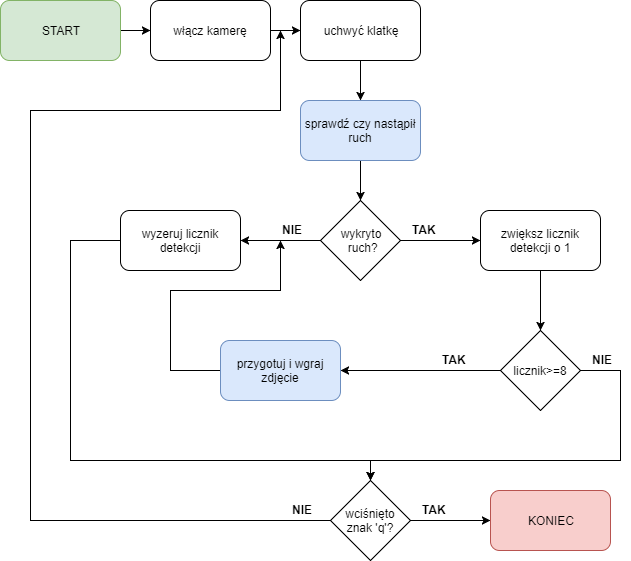
\includegraphics[scale=0.6]{detekcja_ruchu.png}
	\caption{Proces wykrywania ruchu zaimplementowany w aplikacji konsolowej do zarządzania domem}
	\label{fig:proces_detekcji}
\end{figure}

\subsection{Wykrywanie ruchu} \label{ss:wykrywanie}
Proces określający czy od poprzedniego wywołania funkcji nastąpił ruch zaprezentowano na rysunku \ref{fig:wykrywanie_ruchu}/

Na początku wczytane zdjęcie zostaje przeskalowane do szerokości 500px z zachowaniem proporcji wymiarów. W kolejnym kroku obraz zostaje przekonwertowany do skali szarości. Następnie obraz zostaje wygładzony przy pomocy rozmycia gaussowskiego. Jeśli jest to pierwsze uruchomienie funkcji i zmienna przechowująca średnią wartość klatki jest pusta to zostanie do niej przypisany aktualny obraz. Przy pomocy wbudowanej funkcji OpenCv dochodzi do akumulacji w sposób wagowy wartości średniej klatki oraz aktualnej.     

W wyniku tej operacji uzyskany zostaje obraz, na którym widoczne są jedynie obszary różniące się między aktualną klatą, a średnią. Następnie wszelkie braki/wypustki w obrazie zostają wypełnione dzięki dwukrotnie zastosowanej dylatacji strukturą o wymiarach 3x3 px. Ostatnim krokiem jest znalezienie konturów na przetworzonym obrazie, które są końcowym rezultatem działania funkcji.
 \begin{figure}[H]
	\centering
	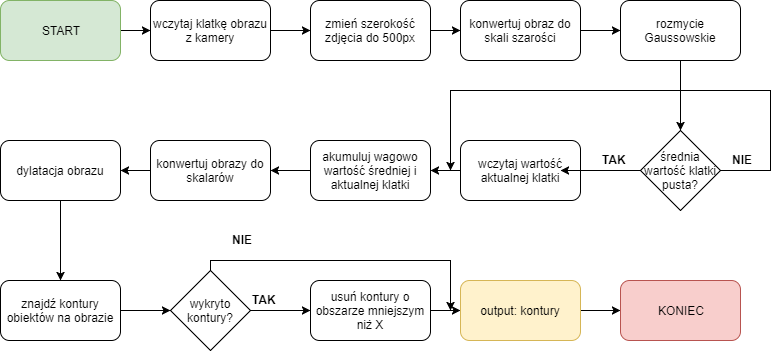
\includegraphics[scale=0.6]{sprawdzenie_ruchu.png}
	\caption{Proces sprawdzenia czy wystąpił ruch zaimplementowany w aplikacji konsolowej do zarządzania domem}
	\label{fig:wykrywanie_ruchu}
\end{figure}

\subsection{Powiadomienie o wykryciu ruchu}
Zgodnie z wcześniej opisanym algorytmem, wykryty ruch zostaje przekazany do zapisania. W zależności od typu aktualnie włączonych opcji, zdjęcie może zostać zapisane w nienaruszonym stanie lub z dodatkowo oznaczoną strefą, w której nastąpił ruch. W kolejnym etapie zostaje utworzony nowy wpis w bazie danych przechowującej informacje o wykrytych ruchach, a zdjęcie zostaje wgrane do odpowiedniego folderu w serwisie Dropbox. Efekt utworzenia nowego wykrycia ruchu można zaobserwować na zdjęciu \ref{fig:notifications}.
